\documentclass[a4paper]{article}
\usepackage[left=1in,right=1in,top=1.2in,bottom=0.85in]{geometry}
\usepackage{mathptmx}
\usepackage{amsmath}
\usepackage{amsfonts}
\usepackage{amsthm}
\usepackage{tikz,pgfplots}
\usepackage{graphics}
\usepackage{bm}
\usepackage{eqlist}
\usepackage{array}
\usepackage{thmbox}
\usepackage{pifont}
\usepackage{tikz-3dplot} %for tikz-3dplot functionality
\usepackage{mathtools}
\usepackage{pgfplotstable}
\usepackage{xintexpr}
\usepackage{romannum}
\usepackage[outline]{contour}\contourlength{1.5pt}
\usepackage{marvosym}
\graphicspath{{.}}
\pgfplotsset{compat=newest}
\usepgfplotslibrary{groupplots}
\usepackage[active,pdftex,tightpage]{preview}
\PreviewEnvironment[]{tikzpicture}
\PreviewEnvironment[]{pgfpicture}
\DeclareSymbolFont{symbolsb}{OMS}{cmsy}{m}{n}
\SetSymbolFont{symbolsb}{bold}{OMS}{cmsy}{b}{n}
\DeclareSymbolFontAlphabet{\mathcal}{symbolsb}



\begin{document}
\begin{tikzpicture}[scale=0.6]

\begin{scope}
\clip(-25.8,-18.1) rectangle(25.8,18);
\node at (0,0){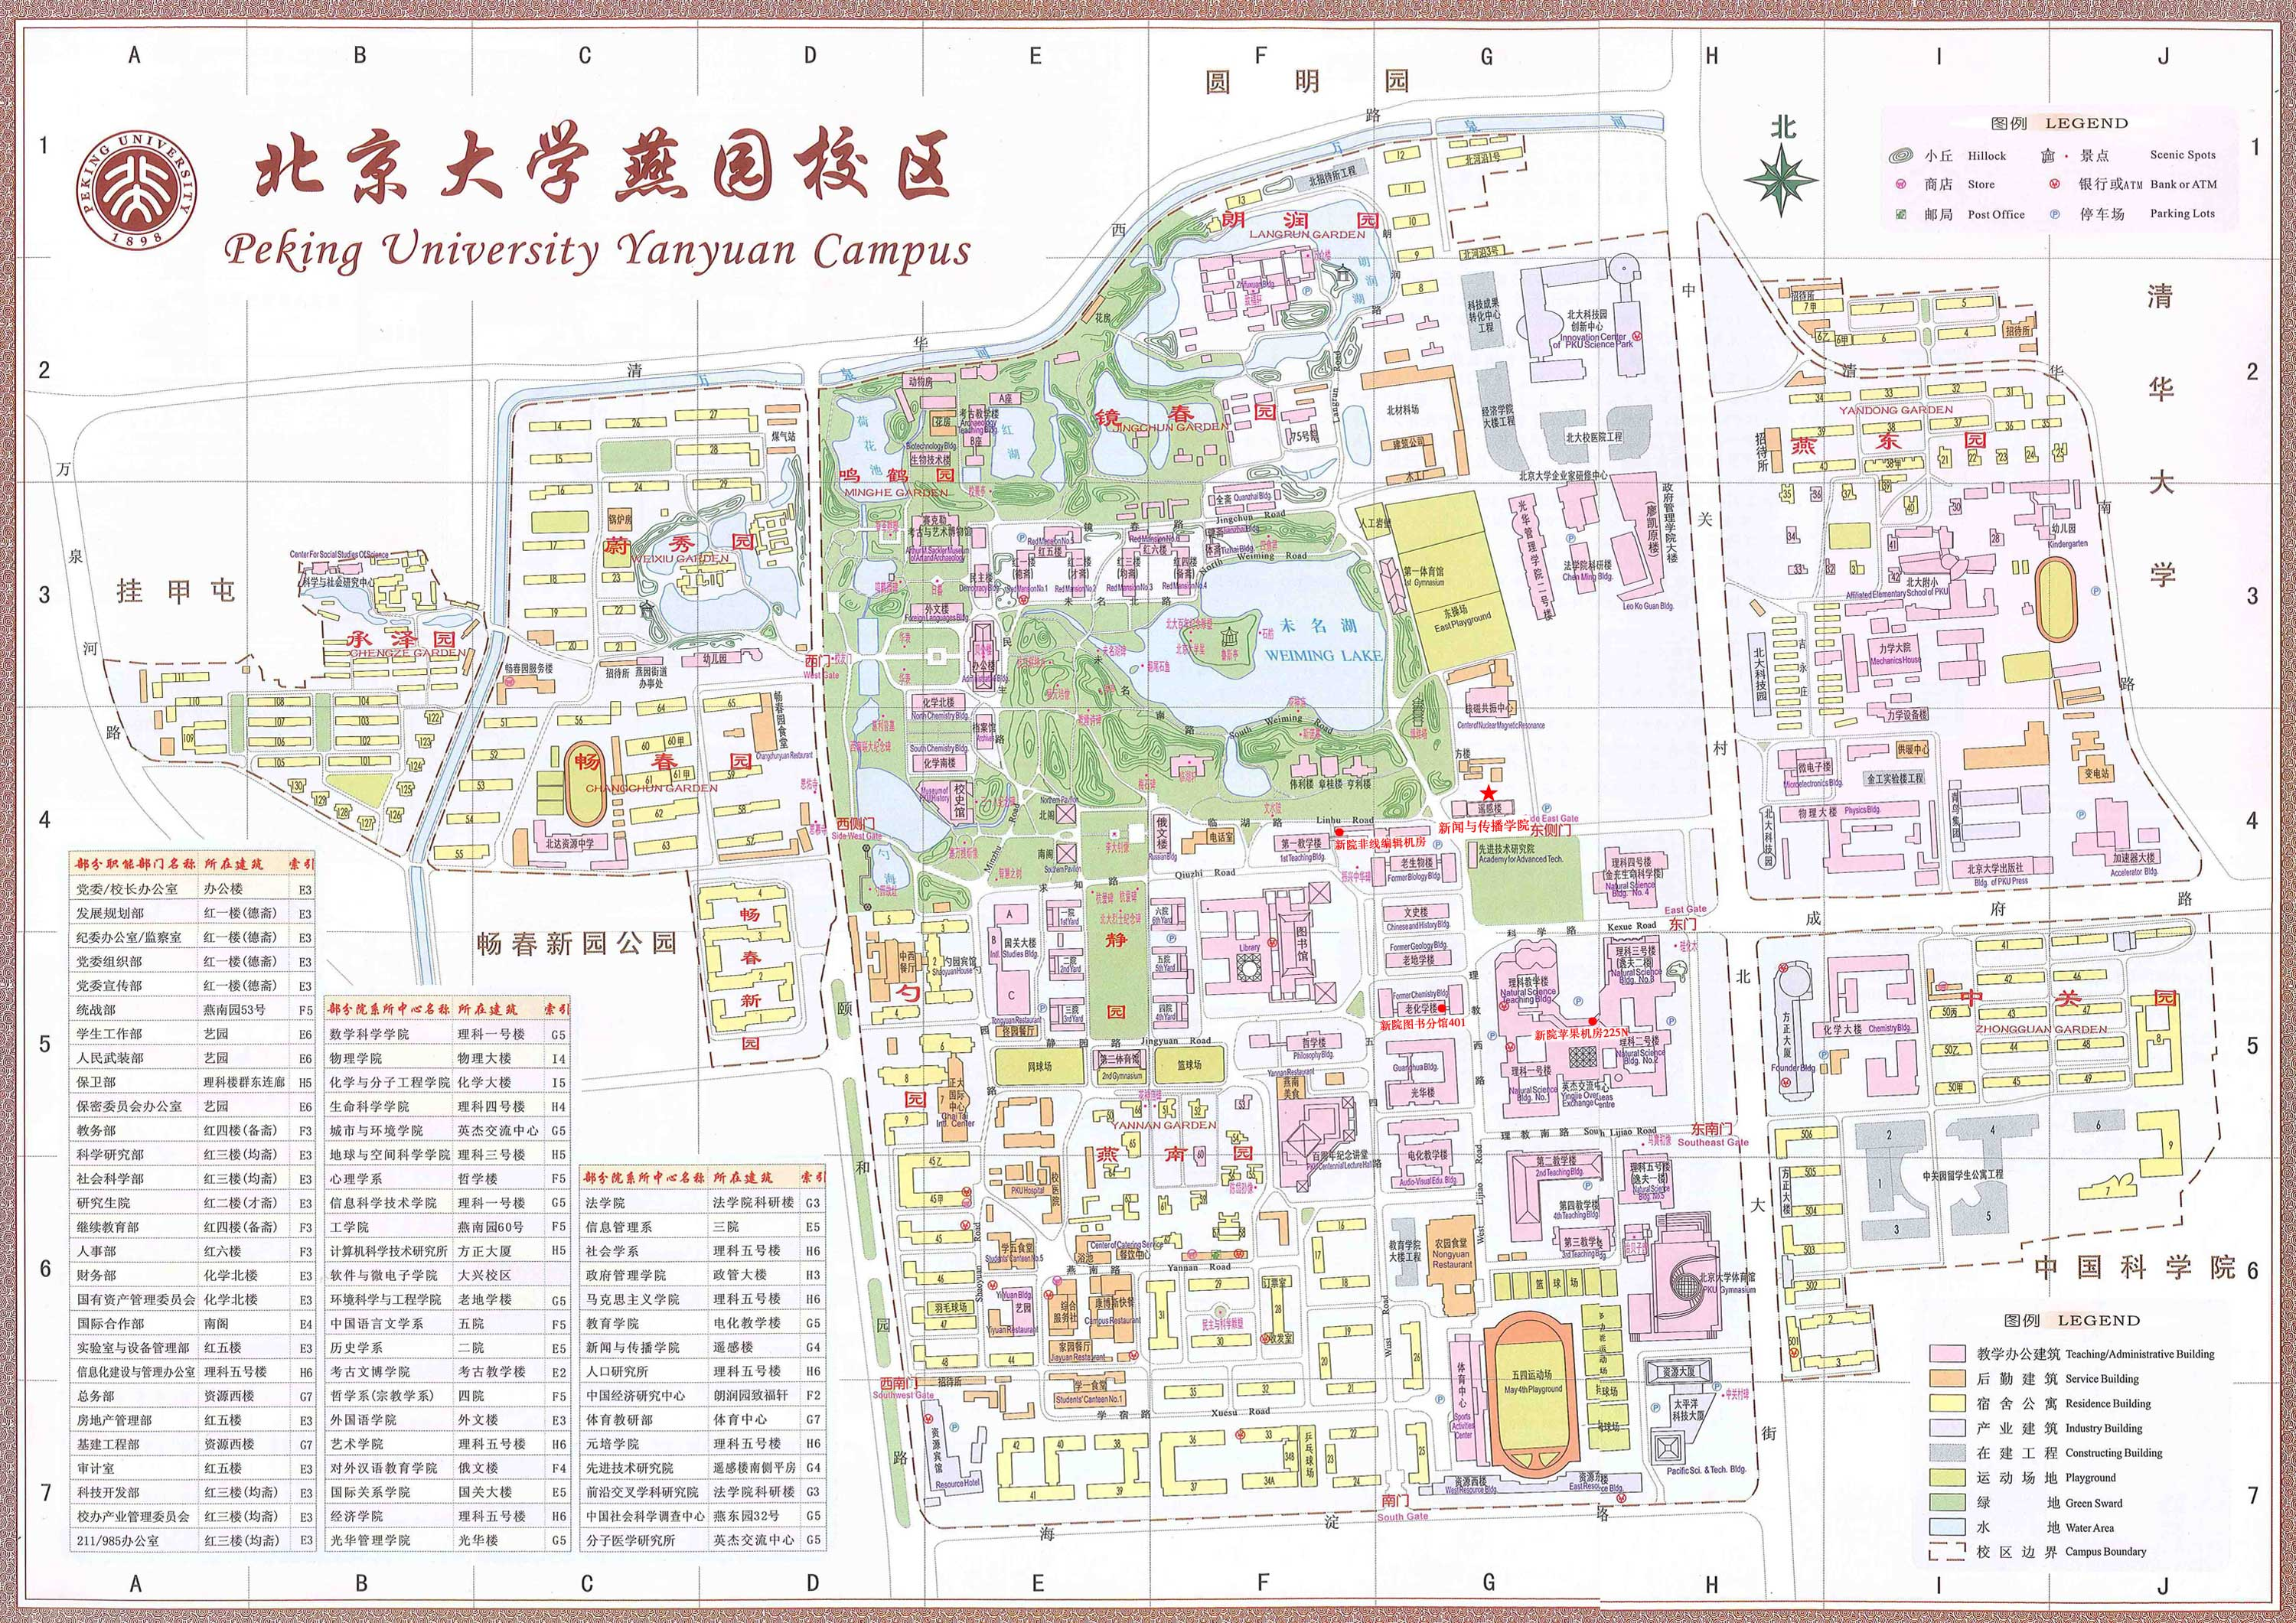
\includegraphics[scale=0.3]{../Dropbox/CASWorks/SPHERIC/figures/PKUmap.jpg}};
\end{scope}

\node[white,shape=circle,fill=red,font=\large\bf,inner sep=1pt,draw=black] at (10,-5.8){A}; 

\node[white,shape=circle,fill=blue,font=\large\bf,inner sep=1pt,draw=black] at (8.8,-6.25){B}; 
\node[white,shape=circle,fill=purple,font=\large\bf,inner sep=1pt,draw=black] at (16.5,-7.5){C}; 

\node[shape=circle,fill=green,font=\large\bf,inner sep=1pt,draw=black] at (16.5,-9){D}; 

\node[shape=circle,fill=green,font=\large\bf,inner sep=1pt,draw=black] at (23,-7.5){E}; 


\draw[thick](-25.8,-18.1) rectangle(25.8,18);


\filldraw[fill=white,draw=black](-25,-17.1)--(-7.4,-17.1)--(-7.4,-7.75)--(-13,-7.75)--(-13,-4.1)--(-19,-4.1)--(-19,-0.75)--(-25,-0.75)--cycle;

\node[right,font=\large] at (-24,-7){A. Yingjie Exchange Center};
\node[right,font=\large] at (-24,-9){B. \#1 Science Blk};
\node[right,font=\large] at (-24,-11){C. Yi Yuan, For buffet lunch};
\node[right,font=\large] at (-24,-13){D. \#1 ZhongGuanYuan Global Village PKU};
\node[right,font=\large] at (-24,-15){E. \#9 ZhongGuanYuan Global Village PKU};


\end{tikzpicture}

\end{document}